\documentclass[11pt]{article}
\usepackage[left=1.3in,right=1.3in,top=1.3in,bottom=1.3in]{geometry}
\usepackage{lipsum}
\usepackage[hidelinks]{hyperref}
\urlstyle{same}
\usepackage{multicol}
\usepackage{footmisc}
\usepackage[toc,page]{appendix}
  
\usepackage{mathtools}
\usepackage{amsmath}
\usepackage{amsfonts}
\usepackage{amssymb}
\usepackage{textcomp}
\usepackage{gensymb}
\usepackage{amsthm}
\usepackage{thmtools}

\theoremstyle{definition}
\newtheorem{defi/}{Definition}[section]

\newenvironment{defi}
  {\renewcommand{\qedsymbol}{$\blacktriangleleft$}%
   \pushQED{\qed}\begin{defi/}}
  {\popQED\end{defi/}}

\newtheorem{theorem/}[defi/]{Theorem}

\newenvironment{theorem}
  {\renewcommand{\qedsymbol}{$\blacktriangleleft$}%
   \pushQED{\qed}\begin{theorem/}}
  {\popQED\end{theorem/}}
  
 \newtheorem{prop}{Proposition}

\usepackage{url}

\usepackage[utf8]{inputenc}

% For nicely formatted header (choose what the left, right and center headers and footers say) (\thepage gives the page number, \leftmark gives section title and \rightmark gives the subsection title)
\usepackage{fancyhdr}
\pagestyle{fancy}
\lhead{}
\chead{}
\rhead{Daniel Widdowson, 201459067}
\lfoot{}
\cfoot{\thepage}
\rfoot{}
\renewcommand{\headrulewidth}{0.4pt}
\renewcommand{\footrulewidth}{0.4pt}
\renewcommand{\thefootnote}{[\arabic{footnote}]}
\setlength{\headheight}{20pt}
\title{Consideration of a new similarity measure for periodic sets}
\author{Daniel Widdowson
\\    \\    \\
A DISSERTATION
\\    \\
Submitted to 
\\    \\    \\ 
The University of Liverpool
\\    \\
\\    \\
in partial fulfilment of the requirements
\\
for the degree of 
\\     \\
MASTER OF SCIENCE
\\     \\    \\    \\
}


\usepackage{sidecap}

\usepackage[
backend=bibtex,
style=alphabetic
]{biblatex}
\addbibresource{references.bib}


\begin{document}

\maketitle
\thispagestyle{empty}

\newpage

\null

\begin{abstract}
This project investigates a specific challenge in computational geometry, the motivation for which lies in crystallography. It was carried out with a general eye towards developing new methods for visualisation, analysis and prediction of crystal structures. The content of this project largely follows from, investigates and attempts to push forward results found in \cite{2020-Mosca-Kurlin, mosca2020average}, though it's intended to be complete enough so there is no prerequisite reading. In the following we will give and explain all basic definitions, lay out the crystal structure prediction problem, introduce definitions and results from \cite{2020-Mosca-Kurlin}, and then attempt to lend consideration to the behaviour of their new measures numerically and mathematically.
\end{abstract}

\null

\section{Setup}

A \emph{unit cell} is a (non-degenerate) parallelipiped in 3D, usually given by three lengths and three angles in a canonical order. A \emph{motif} is then defined as some finite collection of points in the unit cell, and the \emph{periodic set} or \emph{crystal} is then given by repeating the motif periodically in the three directions of the unit cell. Formal definitions are below, extended for any dimension.

\begin{defi}\textsc{lattice, unit cell, motif, periodic set.}\\
\label{def1}
Let $V = \{v_1,v_2,\dots, v_n\}$ be a basis for $\mathbb{R}^n$. A \emph{lattice} $\Lambda$ consists of all linear combinations of $V$ with integer coefficients,
\[
\Lambda = \left\{\sum_{i=1}^n \lambda_iv_i \mid \lambda_i\in \mathbb{Z} \right\}
\]
and the \emph{unit cell} $U$ is the parallelipiped with $v_1,\dots,v_n$ along its edges,
\[
U = \left\{\sum_{i=1}^n \lambda_iv_i \mid \lambda_i\in [0,1) \right\}.
\]
Then, a \emph{motif} $M$ is a finite collection of points in the unit cell, representing a collection of atoms. Finally a \emph{periodic set} $S$ is the natural sum  (\emph{Minkowski sum}) of the lattice and motif, 
\[
S = \Lambda + M = \{u+v \mid u\in \Lambda, v\in M\} \subset \mathbb{R}^n.
\]
From now, the terms `periodic set', `periodic crystal' or just `crystal' may be used interchangeably.
\end{defi}

\subsection{Notes}

The definitions above are formal and general enough to be given in $\mathbb{R}^n$, but since the periodic set represents atoms in 3D space, when it comes to concrete use we are restricted to $\mathbb{R}^3$. 

It may or may not be necessary to specify atomic types, atomic bonds or other information alongside the periodic set. Formally this can be done by either giving the motif as a collection of pairs (position, atomic number) or by ordering the motif and giving a corresponding ordered list of atomic numbers or symbols. Similarly atomic bonds could be given by a list of pairs of positions which are bonded, or pairs of indices for an ordered motif.

The figure below shows a unit cell and motif, where atomic types and bonds are shown, and atoms are not `wrapped' inside the unit cell so that the motif consists of wholly connected molecules. A `wrapped' version of the motif would take all atoms modulo the unit cell so that they all lie inside, resulting in an identical periodic set, but disconnected molecules in the finite motif (if we choose to show bonds).

\begin{figure}[h]
\centering
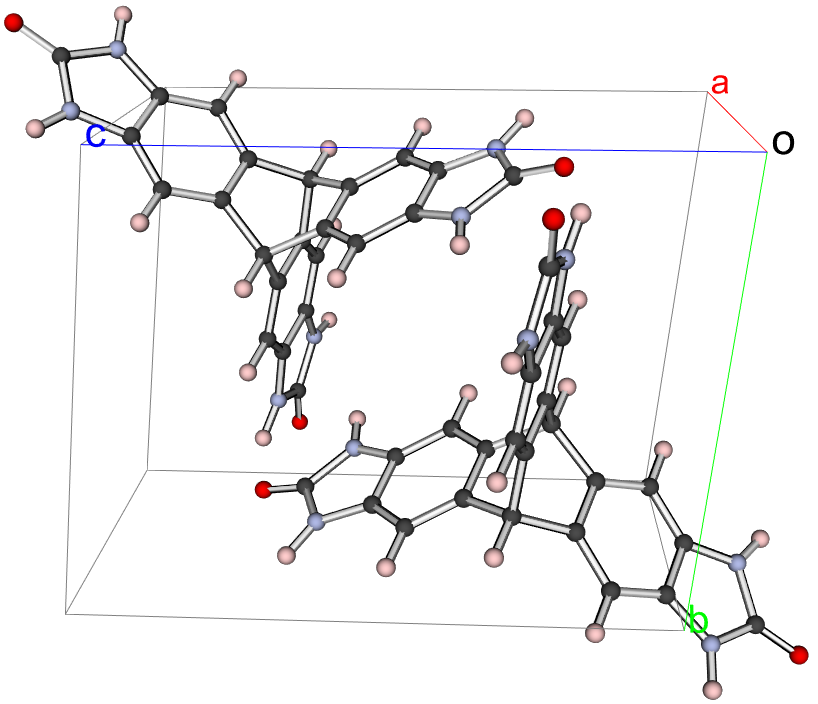
\includegraphics[scale=0.33]{example.png}
\caption{Example unit cell and motif, displayed using a custom renderer in Python. For code see Appendix \ref{app1}.}
\end{figure}

\subsection{CIF file format}

The CIF (Crystallographic Information File) format is a file format developed by IUCr (International Union of Crystallography) designed for storage and exchange of crystallographic and related structural science data. The formal, complete working specification for the CIF format can be found at \cite{CIF}. This project used the format for storage and exchange of crystal data. 

In general, a CIF file defines a unit cell with a canonical list of three lengths $a,b,c$ (in angstroms) and three angles $\alpha,\beta,\gamma$. If $A,B,C$ denotes three sides of the unit cell with $|A|=a, |B|=b$ and $|C|=c$, then $\alpha = \angle BC, \beta = \angle AC$ and $\gamma = \angle AB$. Then a motif is given by a list of \emph{fractional coordinates}, meaning fractions along each of the cell edges, where $(0,0,0)$ is where $A,B$ and $C$ intersect. In other words, fractional coordinates use the edges of the unit cell as a basis. 

CIF files are designed for a wide range of uses, and thus may include much more information (or perhaps less) than just a unit cell and motif. The format is designed towards being general more so than specific. The included data also does not have to abide by particularly strict rules, for example coordinates can specify points outside the unit cell, and need not even be unique modulo the unit cell (even though that is impossible for a real crystal).

CIF parsers used in this project included ase and pymatgen. For the CIF-related code used in this project, see Appendix \ref{app1}.

\section{Crystal Structure Prediction}\label{csp-problem}

\emph{Crystal Structure Prediction} (CSP) is an area of techniques and research aiming to discover new useful (real, synthesizable) crystals. Usually, this is done by simulating atoms in a box, letting them move and settle into a configuration which is stable. By \emph{stable} we mean \emph{thermodynamically stable}, i.e. a low-energy configuration, measured by an energy function. The first issue that arises is that the energy function is complicated and expensive to compute, making this process slow in general as the number and accuracy of the simulations grows.

A supercomputer could spend weeks searching the enormous space of possible crystals to find ones which minimize the energy function. In brief, the goal of the CSP problem is to make the process less expensive in general.

\null

In more detail, current CSP methods return far more crystals at local minima of the energy function than actually exist. What is expected are specific local minima at which a few stable crystals exist, separated by high-energy areas of the function. Instead, we see many crystals in the output which hint towards local minima where a stable crystal may exist.

 The issue is essentially that there is no `good' algorithm known to compare crystals and measure similarity. This means time is spent considering near-identical crystals it can't tell apart, and similarly it doesn't know when two are really different. So, the output of CSP algorithms are post-processed to remove near-identical crystals and separate different crystals, wasting more time (given that methods may exist to solve these problems). 

Note that different unit cells may define geometrically identical crystals, so it is not valid to directly numerically compare two crystals' unit cells or motifs. Another way we might go about comparing crystals is relying on chemistry-related properties. Problems arise when we consider that usually a CSP algorithm is applied to a restricted collection of crystals which don't differ chemically, for instance, all containing the exact same proportions of all atomic types, and in many of these cases crystals can only be distinguished by their geometry, not chemistry.  

\null

We are first required to lay out what exactly should be meant by equivalent or near-equivalent periodic sets. We cannot use unit cell dependent features or fractional coordinates, since these representations for a periodic set are not unique. Instead what is needed is a feature which is \emph{invariant} under transformations which we agree do not alter the crystal. The transformations in question include rotations, translations and reflections; these are rigid motions which don't alter crystals as they are rigid structures. In mathematical terms, we want an \emph{invariant under isometry} (isometry meaning distance-preserving transformation). The ideal solution to the problems laid out would take the following form:

Let $P$ be the space of all periodic sets, and for $S,Q\in P$ let $S\sim Q$ denote that $S$ and $Q$ are isometric. Find a function $f:P\rightarrow N$, where $N$ is some numerical space, such that
\begin{enumerate}
\item $f$ is \emph{invariant under isometry}: $S\sim Q \implies f(S) = f(Q)$,
\item $f$ is \emph{complete with respect to isometry}: $f(S) = f(Q) \implies S \sim Q$,
\item $f$ is \emph{continuous}: small perturbations of points in $S$ results in a small change in $f(S)$,
\item for any $S\in P$, $f(S)$ is \emph{computable} in polynomial time with the motif size of $S$.
\end{enumerate}

Intuitively, an $f$ having all of the above would behave like a `fingerprint' for crystals, where  (1) isometric crystals have the same fingerprint, (2) if two crystals have the same fingerprint they are isometric, and (3) two slightly different crystals have only slightly different fingerprints.

These points (particularly 1) can be summarized mathematically using \emph{equivalence classes}. Briefly (but not precisely), isometry is an \emph{equivalence relation}, meaning it satisfies a set of rules such that $P$ can be split up into disjoint subsets (\emph{equivalence classes}) where any two members of the same class are isometric. This collection of equivalence classes is called a \emph{quotient set}, denoted $P/\sim$. Points 1--3 above can now be summarized by saying there exists a a bi-continuous bijection $\hat{f}: P /\sim \,\, \rightarrow N$, and if $S\in A\in P/\sim$, we have $\hat{f}(A) \eqqcolon f(S)$.

\null

Invariants exist and are used to separate non-isometric crystals from each other, though they do not satisfy all of 1--4 above. Density is a stable isometry invariant which is used but is not complete, symmetry groups are also an invariant but are discrete and unstable. 

A less demanding sub-goal of finding $f$ as above is to find a functions filling the conditions `well enough'. Some measures are better than others because of the degree to which they satisfy 1--4, not because they satisfy more of the points completely. For example mapping all crystals to 0 under $f$ satisfies all points except 2 where it fails so poorly (because $f(S)=f(Q)$ for all $S,Q$) that it is less than poor at separating crystals. Density is `more complete', in that it will at least act as a separator for some crystals. By this standard, any separator better than currently known ones should be considered a success.

In the following sections, we introduce and explore new measures introduced by \cite{2020-Mosca-Kurlin} which have been shown to separate some crystals better than existing methods.

\section{Introducing the Average Minimum Distance}

\subsection{Definitions}\label{defmk20}

\cite{2020-Mosca-Kurlin, mosca2020average} introduced new measures which has potential use in solving the CSP problem. This section will introduce and explain the relevant definitions, most importantly Definition \ref{amd}.

\null

For the following, let $C = \Lambda + M$ be a periodic set, with $M = \{p_1,\dots,p_m\}$ in an arbitrary ordering.

\begin{defi}\textsc{pointwise distribution of distances (pdd).}\\
Let $d^{nn}: M\times \mathbb{N}_{>0} \rightarrow \mathbb{R}$ be the `nearest neighbour distance' function, such that $d^{nn}(p_i, j)$ is the Euclidean distance between $p_i$ and the $j$th nearest neighbour (in $C$) to $p_i$. We will use the abbreviation $d^{nn}_{ij}\coloneqq d^{nn}(p_i,j)$ for brevity. Then, for a fixed integer $k>0$, the \emph{pointwise distribution of distances} PDD$(C;k)$ is the matrix $m\times k$ such that PDD$(C;k)_{ij} = d^{nn}(p_i,j) = d^{nn}_{ij}$,
\[
\text{PDD}(C;k) \coloneqq \begin{pmatrix}
d^{nn}_{11} & d^{nn}_{12} & \dots & d^{nn}_{1k} \\
d^{nn}_{21} & d^{nn}_{22} & \dots & d^{nn}_{2k} \\
\vdots        & \vdots        & \ddots & \vdots \\
d^{nn}_{m1} & d^{nn}_{m2} & \dots & d^{nn}_{mk}
\end{pmatrix}
\]
In other words, each row corresponds to one point in the motif, and the $j$th column corresponds to $j$th nearest neighbour distances for each of the points. \qedhere
\end{defi}

We may think of the PDD as an encoding for the geometric information or relative distribution of points in a periodic set. As defined above, it is still dependent on the ordering chosen for the motif; to remove this dependency we now introduce an ordering for the rows. 

Given the $a$th and $b$th rows, let $(d^{nn}_{aj})_{1\leq j\leq k} < (d^{nn}_{bj})_{1\leq j\leq k}$ if the first (possibly none) entries coincide ($d^{nn}_{aj} = d^{nn}_{bj}$ for $1\leq j\leq \ell$ for some $1\leq \ell\leq k-1$), and the next entry in row $a$ is smaller than that of row $b$ ($d^{nn}_{a,\ell+1}<d^{nn}_{b,\ell+1}$). This is called a \emph{lexicographical} ordering, and choosing this order for the rows of the PDD removes the dependency on the ordering chosen for the motif.

However, the PDD still has dependencies that we would like to remove, particularly the choice of unit cell (and hence number of points in the motif). If we take a periodic set with a unit cell, and then make one edge of the cell twice as long, the periodic set remains the same but the number of motif points doubles, thus doubling the number of rows in the PDD, with each row appearing twice (because the set is periodic). A way to remove repeated rows is now introduced.

\begin{defi}\textsc{weighted point-wise distribution (wpd).}\\
For the $i$th row in PDD$(C;k)$, define the \emph{weight} $w_i$ of the row as the number of times that row appears in PDD$(C;k)$ divided by $m$. More precisely,
\[
w_i \coloneqq \frac{1}{m}\left|\{1\leq j\leq m \,|\, d^{nn}_{jt} = d^{nn}_{it} \text{ for all } 1\leq t\leq k\}\right|.
\]
where $|A|$ is the number of elements of $A$. Then, the \emph{weighted point-wise distribution} WPD$(C;k)$ is PDD$(C;k)$ where each row appears exactly once i.e. identical rows are collapsed into one, and an extra column is appended containing the weight of each row.
\end{defi}

Another way to remove the same dependence the WPD does, as well as summarize the distance distribution information into a simpler metric, is the following (a definition which is the focus of this project).

\begin{defi}\textsc{average minimum distance (amd).}\label{amd}\\
Given a fixed integer $k > 0$, the \emph{average minimum distance} AMD$_k(C)$ is the average of the $k$th column (last column) of PDD$(C;k)$, or equivalently a weighted average of rows in WPD$(C;k)$. If WPD$(C;k)$ has $\ell$ rows with weights $w_1,\dots,w_\ell$,
\[
\text{AMD}_k(C) \coloneqq \frac{1}{m}\sum_{i=1}^m d^{nn}_{ik} = \sum_{i=1}^{\ell}w_i\text{WPD}_{ik}(C;k). \qedhere
\]
\end{defi}

The AMD is `simpler' in the sense that the output space is just $\mathbb{R}$ rather than a space of matrices. 

\subsection{Results}

\cite{2020-Mosca-Kurlin, mosca2020average} proves several results which justify the existence of these measures. These are included but not proven here.

\begin{theorem}\textsc{isometry invariance of the wpd and amd.}\\
The WPD and AMD are invariants under isometry. That is, if $\sim$ denotes isometry between sets, then for any finite or periodic sets $S$ and $Q$,
\[
S \sim Q \implies \text{WPD}(S;k) = \text{WPD}(Q;k) \quad \text{and} \quad \text{AMD}_k(S) = \text{AMD}_k(Q). \qedhere
\]
\end{theorem}

Hence, the WPD and AMD satisfy point 1 in the list in section \ref{csp-problem}. For stability (point 3), we will need some definitions.

\begin{defi}\textsc{bottleneck distance.}\\
For any finite or periodic sets $S,Q$, the \emph{bottleneck distance} BND is
\[
\text{BND}\displaystyle(S,Q) \coloneqq \inf_{\text{bijection } g:S\rightarrow Q}\,\, \sup_{a\in S}|a-g(a)|.\qedhere
\]
\end{defi}

Intuitively, imagine a map $g$ from $S$ to $Q$, then $\sup_{a\in S}|a-g(a)|$ is the largest distance from $a$ to its image under $g$, over all $a\in S$. The BND is the smallest possible value this takes over all bijections $g$. If $Q$ is a slight perturbation of $S$, $g$ will map each point in $S$ to its perturbed point in $Q$, and BND$(S,Q)$ will be largest distance any point was perturbed.

\begin{theorem}\textsc{stability of the amd.}\\
For any finite or periodic sets $S,Q$ and any $k\geq 1$, we have
\[
|\text{AMD}_k(S) - \text{AMD}_k(Q)| \leq 2\text{BND}(S,Q). \qedhere
\]
\end{theorem}

The above can be roughly justified by saying each perturbed point can only move as much as BND$(S,Q)$, therefore pairwise distances between points could have moved no further than twice that.

We will also need a new definition to state that the WPD is stable. The definition (and proof) are more involved since perturbed crystals can have different sized WPDs, so a suitable measure is required to compare such matrices.

\begin{defi}\textsc{earth mover's distance.}\\
Let $S, Q$ be two finite or periodic sets, and $k\geq 1$. For a crystal $S$, denote the $i$th row of WPD$(S;k)$ (without the weight) by $R_i(S)$, the weight of row $R_i(S)$ by $w_i(S)$, and let $m(S)$ be the number of rows in the WPD. Then
\[
\text{EMD}(S,Q) \coloneqq \min_{f_{ij}}\left[\sum_{i=1}^{m(S)} \sum_{j=1}^{m(Q)} f_{ij}|R_i(S) - R_j(Q)| \right]\quad \text{such that}\quad  0\leq f_{ij} \leq 1,
\]
\[
\sum_{j=1}^{m(Q)} f_{ij} = w_i(S) \text{ for } 1\leq i\leq m(S), \quad \text{ and } \quad \sum_{i=1}^{m(S)} f_{ij} = w_j(Q) \text{ for } 1\leq j\leq m(Q).\qedhere
\]
\end{defi}

Intuition for this measure is more difficult to explain quickly, but roughly speaking, the parameters $f_{ij}$ are quantifying a `flow' of moving between rows, $f_{ij}|R_i(S)-R_j(Q)|$ represents a `cost' for flow between rows, and so the EMD is the minimum total cost of moving from one WPD to the other. Importantly, it works as the measure we need for the difference between WPDs. We can now state the stability theorem for WPDs.

\begin{theorem}\textsc{stability of the wpd.}\\
For any finite or periodic sets $S,Q$ and $k\geq 1$, we have 
\[
\text{EMD}(S,Q) \leq 2\sqrt{k}\text{BND}(S,Q).\qedhere
\]
\end{theorem}

It is worth mentioning that the EMD has some computability advantages over the BND; more details on that can be found in \cite{2020-Mosca-Kurlin}. We will end this section with a result that  shows that for at least finite sets, WPDs also satisfy point 2 (completeness) in section \ref{csp-problem}.

\begin{theorem}\textsc{reconstruction of finite sets from wpds modulo isometry.}\\
If $S$ is a finite set with $m$ points such that all pairwise distances between points in $S$ are distinct, then $S$ can be reconstructed modulo isometry from WPD$(S;m-1)$. 
\end{theorem}

This shows completeness because if two sets have the same WPD, their reconstructions will be the same modulo isometry. It is conjectured that the above theorem also holds for periodic sets, depending on the complexity of the set and large enough $k$.

\newpage

\section{Numerical Treatment}

For any and all code relevant to this section or others, see Appendix \ref{app1}.

\subsection{Data Acquisition}\label{data-acq}

AMD data used in this project was provided by the authors of \cite{2020-Mosca-Kurlin}. Specifically, the set consisted of the values of AMD$(k)$ for $1\leq k \leq 1000$ across 5679 crystals, one of which was an erroneous enough entry to be excluded, so the total number of crystals considered was 5678. These crystals are those initially reported in \cite{Nature}.

The set of crystals was somewhat homogeneous, in the sense that there was only one unique molecule across the whole set. Still, crystals often had different numbers of this molecule in their motif and each had a unique motif, so it is expected to be a good example to extend to other crystals. The molecule in question is dubbed `T2' and is shown below.

\begin{figure}[h]
\centering
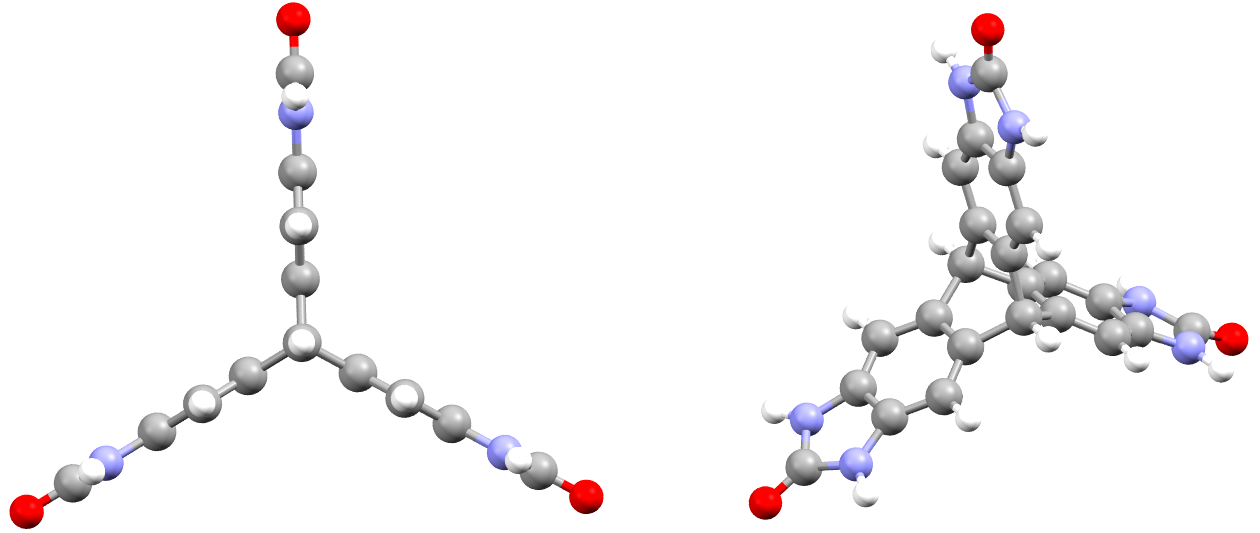
\includegraphics[scale=0.33]{job_03351.png}
\caption{A T2 molecule from two angles, rendered in Mercury. More information on this molecule in \cite{T2}.}
\end{figure}

\subsection{AMD plots}

The main results from this project regard the AMD measure. While the WPD has advantages, at least for fulfilling the aims laid out in section \ref{csp-problem}, AMDs have the advantage that it's simpler measure so it's easier to run experiments and get results. For a given periodic set $S$, the AMD is a function AMD$:\mathbb{N}_{> 0} \rightarrow \mathbb{R}$ which it is natural to plot. 

\begin{figure}[h]
\centering
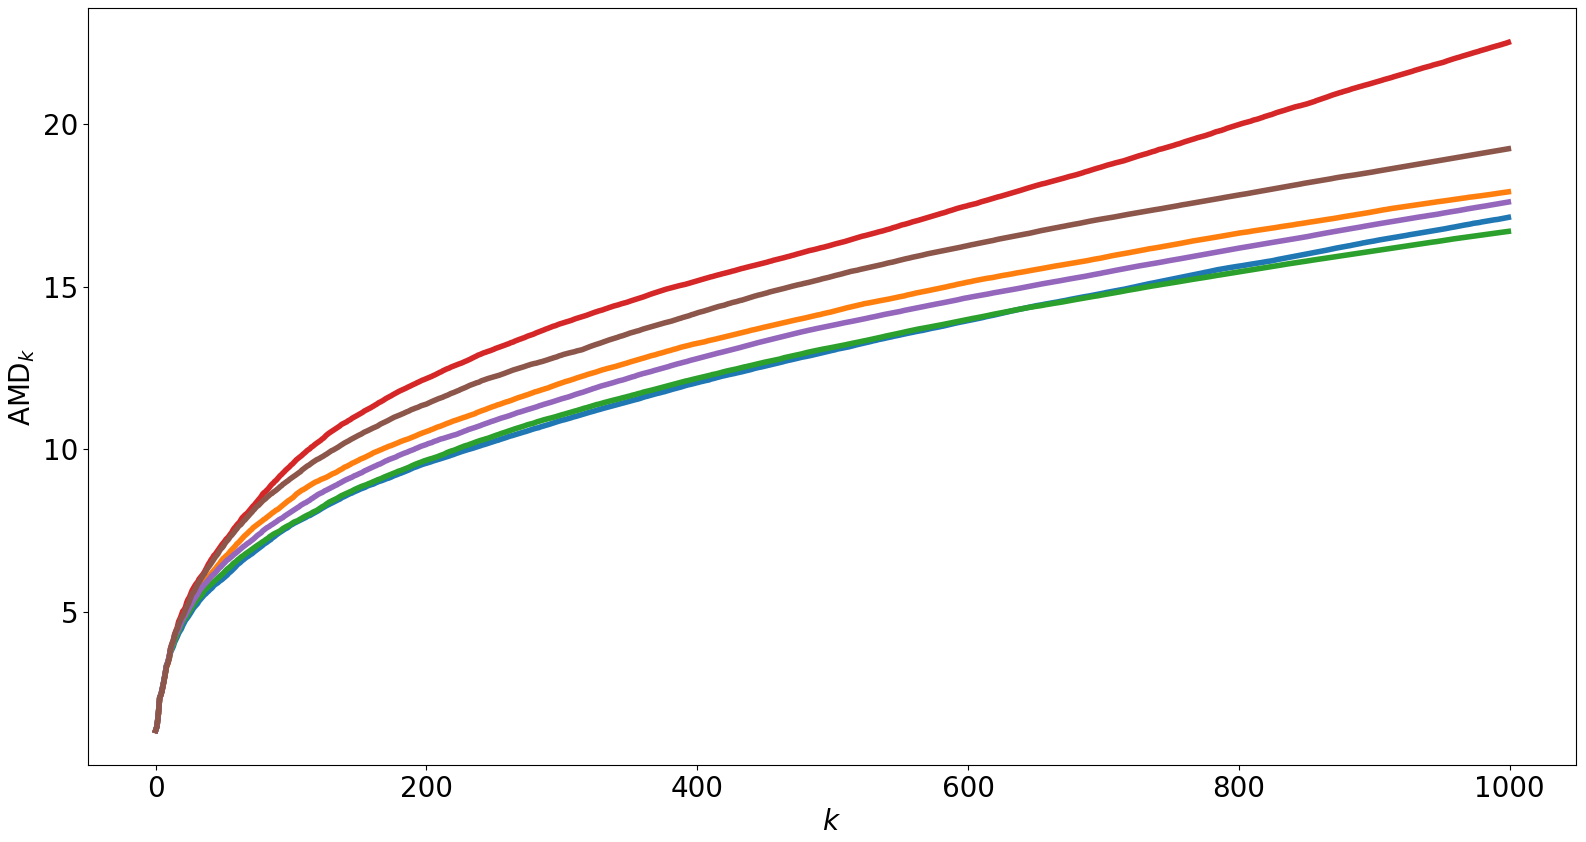
\includegraphics[scale=0.28]{amds2.png}
\caption{AMD$_k$ for 6 randomly chosen crystals, $1\leq k\leq 1000$.}
\label{fig:amd-curves}
\end{figure}

Figure \ref{fig:amd-curves} shows AMD$_k$ for $1\leq k \leq 1000$, for $6$ crystals chosen at random (from the set described in section \ref{data-acq}). Quickly we notice the behaviour is coherent in some sense, but not entirely smooth and predictable. For example, even though curves seem to separate themselves out nicely, one curve may be greater than another for all $k$ up to at least $600$ and then switch the other way (the blue and green curves). In addition, the red curve seems to have a very steady growth rate like the others but that rate suddenly increases at around $k=500$.

\subsection{Fitting}

We turn our attention to pinning down the behaviour of these curves, experimentally. We use the  well-known Python library Scipy \cite{2020SciPy-NMeth}, specifically its curve fitting capabilities. The function \texttt{scipy.optimize.curve\_fit()} was used for the curve fitting; it works as follows.

The function requires three parameters: \texttt{curve\_fit(function, x\_data, y\_data)}, and can accept additional optional parameters. Loosely speaking, \texttt{function} is a Python function which will take \texttt{x\_data} as the first parameter and has additional free parameters, and \texttt{curve\_fit} attempts to minimize the difference between the output of \texttt{function(x\_data, ...)} and \texttt{y\_data} by adjusting the free parameters of \texttt{function}. 

More specifically, \texttt{function} must be a Python callable which takes the independent variable \texttt{x\_data} as its first argument. Remaining arguments are the parameters to be fitted. \texttt{x\_data} and \texttt{y\_data} should be array-like objects, such that \texttt{function(x\_data, ...).shape == y\_data.shape}, i.e. \texttt{function} outputs an array of the same shape as \texttt{y\_data} so they can be compared. \texttt{curve\_fit} uses non-linear least squares optimization to fit the function to the data (passing to \texttt{scipy.optimize.least\_squares}).

\null

Many functions were tried. Before discussion, all the relevant results are shown in Table \ref{fit-table} below. $k$ is used as the independent variable (\texttt{x\_data}), and the rest are free parameters. Briefly, RMS and STD are both measures of how well all the 5678 curves were fit by each function.

\begin{table}[h]
\centering
\begin{tabular}{l|l|l}
function & RMS & STD \\ \hline
$(ak)^{1/3}$         & $0.18165$ & $0.10338$ \\
$(a+bk)^{1/3}$         & $0.17039$ & $0.09620$ \\
$a+(bk)^{1/3}$         & $0.11564$ & $0.07035$ \\
$(ak)^p$         & $0.09899$ &  $0.06459$ \\
$ak^p$         & $0.09899$ & $0.06459$ \\
$a+(b+ck)^{1/3}$         & $0.09885$ & $0.06263$ \\
$(a+bk)^p$         & $0.09015$ & $0.05775$ 
\end{tabular}
\begin{tabular}{l|l|l}
function & RMS & STD \\ \hline
$a+bk^p$         & $0.08025$ & $0.05398$ \\
$a+b(c+dk)^p$         & $0.06696$ & $0.04511$ \\
$a+bk^p+ck^q$         & $0.06040$ & $0.04215$ \\
$a+bk^p+c\log k$         & $0.04957$ & $0.03513$ \\
$a+bk^p+ck^q+d\log k$         & $0.04499$ & $0.03245$ \\
$a+bk^p+c\log (k+d)$         & $0.03996$ & $0.02694$ \\
$a+bk^p+ck^q+d\log (k+e)$         & $0.04977$ & $0.03697$ 
\end{tabular}
\caption{Results of fitting the AMD curves.}
\label{fit-table}
\end{table}

Here, RMS means `average root mean square', given by averaging $\frac{1}{n}\sum_k (\text{AMD}_k - f(k))^2$ across all crystals in the set, where $k$ ranges between 1 and 1000, and $f$ is the function which was fitted to each AMD curve. STD means `average standard deviation of absolute errors', which is the standard deviation of $|\text{AMD}_k - f(k)|$ across all $k$, again averaged across all crystals. They are both included here for completeness but seem to measure error similarly as the two measures seem to line up in proportion for all the functions.

\subsection{Discussion}\label{discussion}

A quick glance at the curves (Figure \ref{fig:amd-curves}) gives away some clues regarding the behaviour: that AMD$_k$ is strictly increasing with $k$, and that the derivative is very large for small $k$, decreasing as $k$ increases, at a rate which slows when $k$ gets large. 

Logarithmic behaviour probably does not play a role because they have the distinctive property that the curve goes to negative infinity when approaching zero, and these curves seem not to. That being said, log functions were included in the results to some interest. 

The other suspect is some kind of root-like behaviour, that is, AMD$_k$ follows a function like $k^p$ for some $p\in (0,1)$, since this family of functions matches the properties we see in Figure \ref{fig:amd-curves}. The results supported this type of function being involved. 

\null

Choosing the `correct' function out of the table (if it's there) needs some careful consideration. Naturally, allowing more free parameters lowers the error, so we should demand that more free parameters lowers the error considerably, so that the parameters chosen were more likely to be natural. 

A good example is the pair $(a+bk)^{1/3}$ and $a+(bk)^{1/3}$, the latter having a much lower RMS. This probably suggests the latter is a closer guess to a good approximation. In practice, it  essentially just rules out the former as a candidate.

In the same way, $a+(bk)^p$ works better than $(a+bk)^p$. Allowing the power $p$ to vary freely allowed the RMS to drop by a non-trivial amount---the only equation without $p$ which beat any one with $p$ was $a+(b+ck)^{1/3}$ which narrowly surpassed $ak^p$. In this case $ak^p$ is still superior because it uses one less free parameter and the RMS change is negligible. 

Allowing $p$ to change leads to a lower RMS, probably because $p$ is strongly responsible for asymptotic behaviour as compared to adding or multiplying by different constants. Similarly, adding more terms like this as in $a+bk^p+ck^q$ just helps the curve fit algorithm control the behaviour much better, but this is unlikely to be a `true' approximation. On that note, it was surprising that adding a log term instead ($a+bk^p+c\log k$) gave a much lower RMS. For these cases and others with more parameters, they were included for completeness rather than being presented as the `correct' choice. 

Speaking of adding many free parameters, the last function is included to demonstrate the upper limit of the curve fitting---notice that the second-to-last has a \emph{smaller} error despite being a subset of the function family after it. This is likely because \texttt{curve\_fit} is hitting an upper limit, it's just much easier to search lower-dimensional spaces for local minima (not to mention that \texttt{curve\_fit} seems to run exponentially slower with more parameters, and at $7$ fitting all $\sim 6000$ curves takes several hours). 

\null

More evidence of interesting behaviour emerges when looking for correlations in the free parameters, graph below.

\begin{figure}[h]
\centering
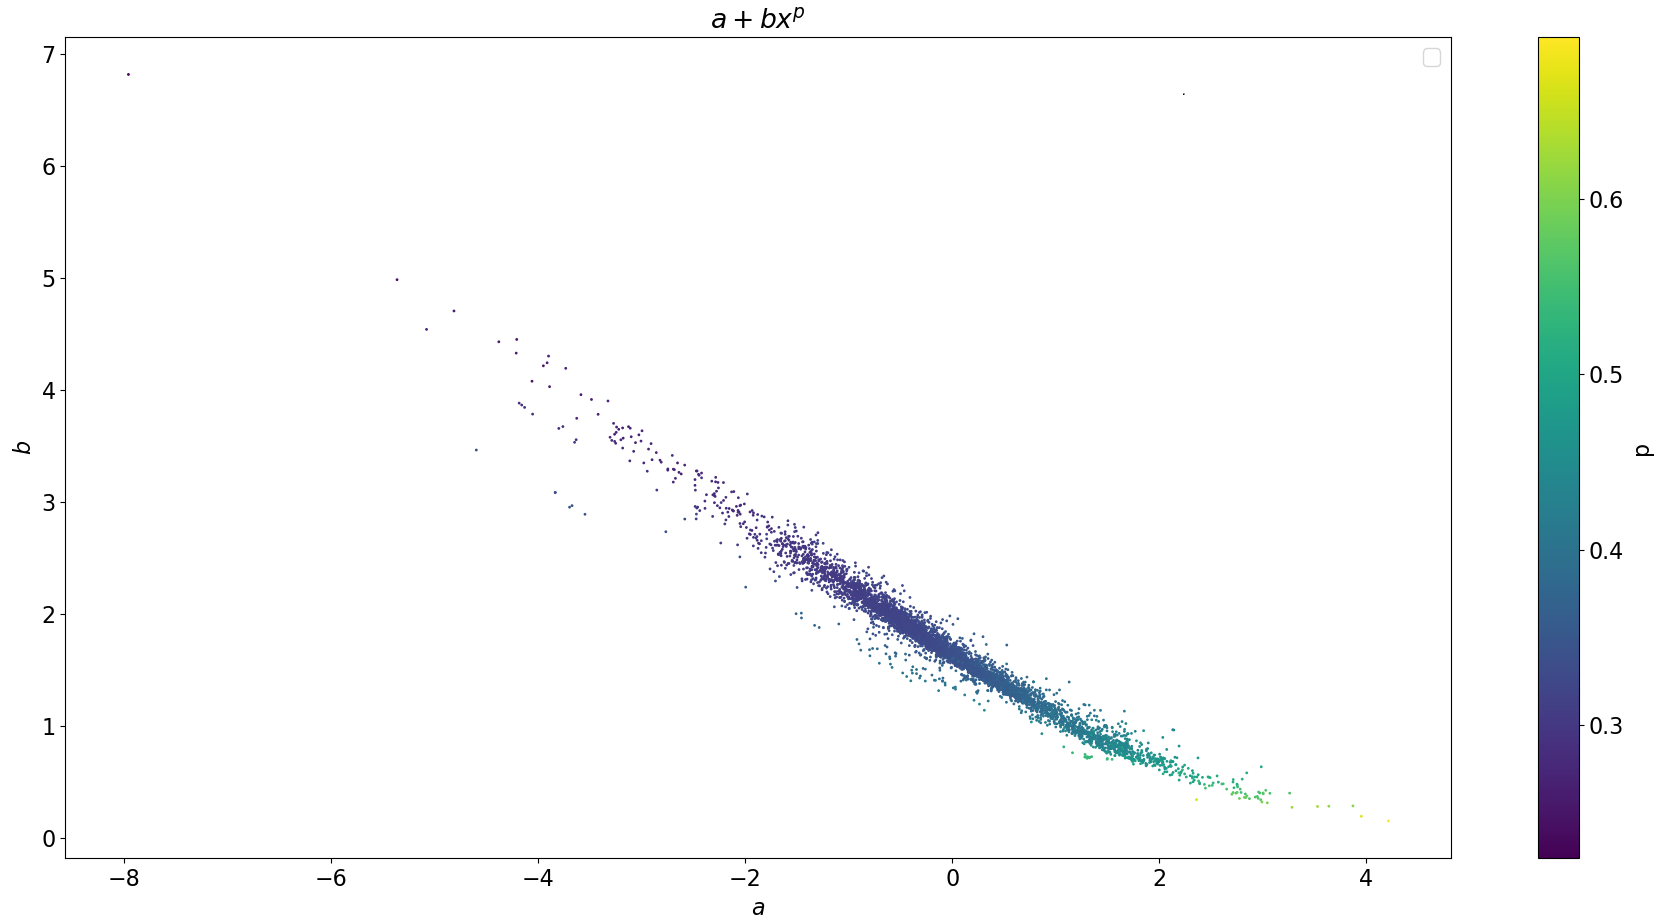
\includegraphics[scale=0.33]{p_scatter_lrg.png}
\caption{Scatter plot for each the $\sim 6000$ crystals' fitted parameters for $a+bk^p$; $a$ on the $x$-axis, $b$ on the $y$-axis and coloured by $p$.}
\end{figure}

The correlations suggest that relationships exist between the parameters. Or further, it suggests that all the curves are related in some way such that finding parameters to fit the curves results in a narrow band of good choices. 

No conclusion is given here about which function most correctly matches the behaviour of the curves. A good guess would be to assume it lies somewhere between many parameters (and a good fit) and few (with a worse fit, but good given the number of parameters).

We end the discussion with a note regarding a potential problem. The maximum $k$ available was $1000$, however the motifs were often almost as large. Given the discussion later in Section \ref{>1dim}, we might expect asymptotic behaviour to emerge when $k/|M|$ (where $|M|$ is the motif size) is suitably large, however in this set $100<|M|<500$ was very common and in some cases $|M|$ exceeded $1000$. No firm conclusion is reached about whether $k=1000$ is big enough---a glance at the graphs indicates no such problem exists.

\subsection{More Attempts}\label{more-attempts}

This subsection covers routes that were attempted, the results of which are only worthy of brief discussion. 

One way to make a compromise with allowing too many free parameters is to allow them to exist in the equations as constants across all the crystals, i.e. for $a+bk^p$ we find the best value of $a$ for all crystals rather than letting it be free for every one. This can be done similarly to before with an optimizer. This time the function we have to optimize takes $a$ as a free parameter, fits all the curves with the given $a$ allowing $b$ and $p$ to vary, and returns the average RMS. The optimizer will find the best constant $a$ to use across all the crystals, eliminating a free parameter. This approach didn't produce too many noteworthy results, but we will note that for equations with a power of $1/3$, a better power can be found but it is close: $(ak)^{0.3508}$ has (slightly) lower RMS than $(ak)^{1/3}$.

\null

Another similar way to eliminate parameters, is to use the correlations mentioned in the previous section. Given that $a,b$ and $p$ are correlated, it could be possible to find $a,b$ or $p$ as functions of the other variables and if the curves still fit reasonably well we have eliminated a degree of freedom. Where this was tried, the error increased by an amount too large to claim any success.

\section{Mathematical Treatment}

\begin{prop}
Let $S=\Lambda+M$ be a periodic set ($n$-dimensional). Let $B(r,p)$ denote the ($n$-dimensional) open ball radius $r$ centered at $p$. Then
\begin{align}
\text{AMD}_k(\Lambda) = \sup \{r \,\,|\,\, |B(r,0) \cap \Lambda| \leq k\}
\end{align}
and more generally
\begin{align}
\text{AMD}_k(S) = \frac{1}{|M|}\sum_{m\in M}\sup \{r \,\,|\,\, |B(r,m) \cap S| \leq k\}
\end{align}
\end{prop}

\begin{proof}

(1) In this simpler case, there is no motif $M$ and the only points in the set are the integer multiples of the basis defining $\Lambda$ (Definition \ref{def1}). Since the PDD and WPD contain only one row, AMD$_k$ is just the distance to the $k$th nearest neighbour to the origin. Let $p(k)\in\Lambda$ denote the point which is the $k$th nearest neighbour to the origin (so, AMD$_k = |p(k)|$, Euclidean distance). Then, the open ball $B(|p(k)|,0)$ contains no more than $k$ lattice points, $|B(|p(k)|,0)\cap \Lambda|\leq k$:

Suppose $|B(|p(k)|,0)\cap \Lambda|>k$. Then, every point in $B(|p(k)|,0)\cap \Lambda$ (excluding the origin itself) would be a nearer neighbour to $0$ than $p(k)$. Removing the origin, there are at least $k$ points closer to the origin than $p(k)$, defined to be the $k$th nearest neighbour.

But, if $\varepsilon>0$ then $|B(|p(k)|+\varepsilon,0)\cap \Lambda| > k$. Adding any $\varepsilon$ to the radius of the ball, it now contains $p(k)\in\Lambda$. The ball must contain at least $k$ nearest neighbours to the origin and the origin itself, so the intersection is at least $k+1$ (it may be larger even for arbitrarily small $\varepsilon$, if multiple lattice points have the same magnitude).

Since we have
\[
|B(|p(k)|,0)\cap \Lambda|\leq k \quad \text{and} \quad |B(|p(k)|+\varepsilon,0)\cap \Lambda| > k \quad \text{for all $\varepsilon$}
\]
we can say AMD$_k = |p(k)| = \sup \{r \,\mid \, |B(r,0)\cap \Lambda| \leq k\}$, this is the supremum of all values of $r$ for which the ball has $k$ or fewer lattice points, which is exactly up until $|p(k)|$.

\null 

(2) The second case is similar, except we are taking an average over all the motif points and the ball is centered at $m\in M$. The argument is the same as in (1), now we pick an arbitrary $m\in M$ and the argument shows that the $k$th nearest neighbour distance from $m$ is 
\[
\sup \{r \,\mid \, |B(r,m)\cap S| \leq k\}
\]
so taking the average over all points in $M$ yields the equation.
\end{proof}

Really this has just reformulated the definition of `$k$th nearest neighbour to $p$' in terms of a ball centered at $p$. In the notation of Section \ref{defmk20}, we could write
\[
d^{nn}_{mk} = \sup \{r \,\,|\,\, |B(r,m) \cap S| \leq k\}
\]

We can equivalently express (1) or (2) using the closed ball $\overline{B}(r,p)$ using the same argument (now, $\overline{B}(|p(k)|,0)\cap S$ contains $p(k)$ and so has at least $k+1$ points, and $\overline{B}(|p(k)|-\varepsilon,0)\cap S$ contains no more than $k$ points or else there are $k$ nearer neighbours to $0$ than $p(k)$). Again by the same arguments we can use the infimum,
\[
\text{AMD}_k(S) = \frac{1}{|M|}\sum_{m\in M}\inf \{r \,\,|\,\, |B(r,m) \cap S| > k\}
\]

In another notation, consider the function $N(S;r,p) = |B(r,p)\cap S|$, the number of points of $S$ inside an open ball radius $r$ centered at $p$. Plugging into (2) we have
\[
\text{AMD}_k(S) = \frac{1}{|M|}\sum_{m\in M}\sup \{r \, \mid \,N(S;r,m) \leq k\}
\]
Fixing $S$ and a point $m\in M$, the expression $\sup \{r \, \mid \,N(S;r,m) \leq k\}$ is essentially the inverse of $N(r):\mathbb{R}\rightarrow \mathbb{N}$; if $N(r)$ takes a radius and gives the number of points inside a ball of that radius, then the inverse would take a number of points $k$ and give the radius such that there are $k$ points inside the ball. We can't exactly take the inverse, since $N$ is not injective and it may change by more than 1 under arbitrarily small changes in $r$. For example, in 2 dimensions if $S = \mathbb{Z}^2$, $N(1) = 1$ as the open circle radius 1 contains just the origin, but $N(1+\varepsilon) = 5$ for small $\varepsilon$, as the circle includes $(1,0), (0,1), (-1,0)$ and $(0,-1)$ (and so, $N^{-1}(2)=\emptyset$). Taking the supremum of $r$ over all balls containing $\leq k$ points accounts for this; $k$ will be mapped to the distance to the $k$th nearest neighbour. 

\subsection{1-dimensional case}

We now consider the simplest case for $S$, in 1 dimension with no motif. In this case we can obtain exact expressions.

\begin{prop} For a 1 dimensional lattice $\Lambda = \{v\}$, we have
\[
\text{AMD}_k(\Lambda) = \left\lceil \frac{k}{2} \right\rceil v
\]
(where $\lfloor x \rfloor$ rounds $x$ down the the nearest integer, and $\lceil x \rceil$ rounds up).
\end{prop}

\begin{proof}
A lattice in 1 dimension is a simple structure, just points on a number line spaced evenly ($v$ apart) and a point at $0$. If a ball has radius $r$, it contains $2\lfloor r/v\rfloor + 1$ points (2 for each side of 0, $+1$ for the origin itself). We can reason directly for the AMD as well, since nearest neighbours to 0 in order are clearly $v,-v,2v,-2v,3v,-3v,\dots$ so the distance to the $k$th nearest neighbour will be $\lceil\frac{k}{2}\rceil v$.
\end{proof}

Now attempting to add a motif $M$, things are a bit trickier.

\begin{prop} For $1$-dimensional $S = \Lambda + M$ with $\Lambda = \{v\}$, 
\[
\left\lfloor \frac{k}{2|M|} \right\rfloor v \leq \sup \{r \,\mid \, |B(r,0)\cap S| \leq k\} \leq   \left\lceil \frac{k+1}{2|M|} \right\rceil v
\]
\end{prop}
\begin{proof}
The ball $B(tv,0)$ for $t\in\mathbb{Z}$ contains these exactly $2t$ copies of the motif (for each side of 0). So
\[
|B(tv,0)\cap S| = 2t|M|
\]
Choosing $t$ so that $2t|M|\leq k$ yields a $r = tv$ with $|B(r,0)\cap S|\leq k$ , so $tv$ is a lower bound for the supremum. The largest valid $t$ is then $t = \lfloor \frac{k}{2|M|}\rfloor$, giving us one bound. The same argument works for the upper bound, except if $2t|M| = k$ exactly then $t = \frac{k}{2|M|}$ is an integer and rounding $t$ up means $|B(tv,0)\cap S|$ still contains exactly $k$ points. To guarantee the intersection is larger than $k$, we can take $t$ such that $2t|M| \geq k+1$, so $t = \lceil\frac{k+1}{2|M|}\rceil$ works for an upper bound.
\end{proof}

The bounds are quite good in that for the most extreme choice of $M$, where there are many points at or near zero, they can be near or equal to the actual value. However for an evenly distributed motif they are often quite bad numerical approximations to $\sup \{r \,\mid \, |B(r,0)\cap S| \leq k\}$. This is because if we expect the bounds to hold for any motif, they will necessarily be quite loose. A good approximation may be to basically assume the motif is uniformly distributed, with
\[
\sup \{r \,\mid \, |B(r,0)\cap S| \leq k\} \simeq \frac{kv}{2|M|}
\]

The approximation here comes from the idea that the ball $B(tv,0)$ contains $2t|M|$ points (for $t\in\mathbb{Z}$). For the AMD, the ball is centered at $m\in M$---in this case we imagine translating the motif to $M - m = \{p-m \mid p\in M\}$ so $m$ moves to $0$, then taking the modulus: $\{p-m \mod v \mid p\in M\}\subset [0,v)$. The nearest neighbours of $m$ are equivalent to the nearest neighbours of $0$ using this as the motif, but since the motif size has not changed, we can use the same approximation as before. Hence the conjectured approximation is AMD$_k \simeq \frac{kv}{2|M|}$, see Figure \ref{amd-line} below.

\begin{figure}[h]
\centering
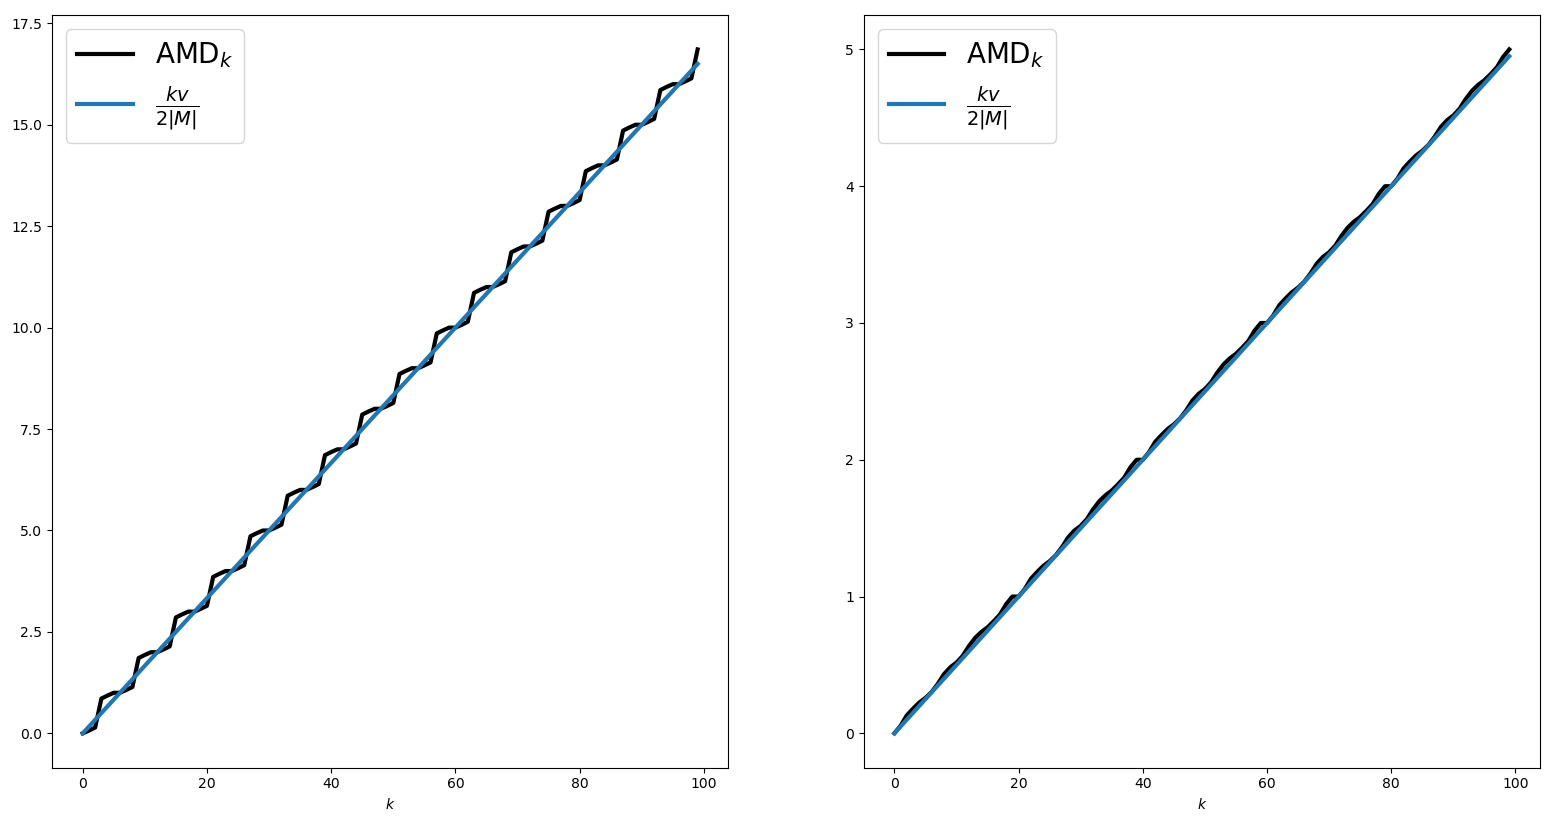
\includegraphics[scale=0.36]{subplots.png}
\caption{Two examples of AMD$_k$ in one dimension and the approximation $\frac{kv}{2|M|}$, for $1\leq k\leq 100$. Both have randomly chosen motifs and $v=1$, left has $|M|=3$ and right has $|M|=10$.}
\label{amd-line}
\end{figure}

\subsection{$> 1$ dimensions} \label{>1dim}

The function $N$ was partly introduced to tie this problem to an existing one. The \emph{Gauss circle problem} is well studied: \emph{given a circle in $\mathbb{R}^2$ radius $r$ centered at the origin, how many points $(m,n)$ are inside the circle where $m,n\in\mathbb{Z}?$} This question asks for the function $N(r) = |\{B(r,0) \cap \mathbb{Z}^2\}|$, and so its `inverse' is $\sup\{r \,\mid \, |\{B(r,0) \cap \mathbb{Z}^2\}|\leq k\}=$ AMD$_k(\mathbb{Z}^2)$. 

The lack of a easy formula for $N(r)$ would indicate it will be difficult to obtain a simple exact formula for AMD$_k$, even more so when introducing a motif. However approximations exist: since each square on the plane contains one lattice point on average, $N(r)$ is approximately the area $\pi r^2$. Gauss showed \cite{GHH} that the error term $E(r)$ has $|E(r)|\leq 2\sqrt{2}r$, and bounds have since improved. Similarly in $n$ dimensions, $|\{B(r,0) \cap \mathbb{Z}^n\}|\simeq \text{Vol}(B(r,0))$.

We can attempt to extend the area idea as follows. The number of unit cells spanned by a basis for $\mathbb{R}^n$ $\{v_i\}_{1\leq i \leq n}$ which lie in the ball $B(r,0)$ will approximately be the volume divided by $\det [v_1\dots v_n] \eqqcolon |U|$, the volume of the unit cell. The number of points in the ball is roughly this multiplied by $|M|$. Making the same assumptions as in 1 dimension,
\[
|\{B(r,0)\cap S\}| \simeq \frac{|M| \text{Vol}(B(r,0))}{|U|}
\]
in the 1 dimensional case, the volume of the ball is $2r$ and we get the approximation from the last section. In 2 and 3 dimensions respectively, we have
\[
r \simeq \sqrt{\frac{k|U|}{\pi |M|}} \qquad r \simeq \sqrt[3]{\frac{3k|U|}{4\pi |M|}} 
\]
We can note here that $|U|/|M|$ is the density of points in the unit cell, as was $v/|M|$ in the last section.

Much more on the (generalised) Gauss circle problem can be found at \cite{point-dist}, which gives a formula and a bound on the error on the number of lattice points in a sphere in any dimension for certain lattices.

The approximation should be better when the ball is large and contains many copies of the unit cell, which ties into the problem explained in Section \ref{discussion}. In Figure \ref{amd-line}, we see oscillations around the AMD line which have a period dependent on $|M|$, so for a better long-term look we let $k$ be big enough to cover many copies of the motif. In the data from Section \ref{data-acq}, the maximum $k$ was $1000$ and $|M|$ could be greater than 1000 (most between 100 and 500), so it may be that $k$ is too small to see asymptotic behaviour. Based on the data and everything considered, though, it is likely that $k=1000$ is large enough and instead the above approximations are missing something. 

At this time more work is needed to find a numerical match between AMD values and approximations we can make via the above equations. While not massively different in behaviour, the approximations above alone are quite distant from actual AMD curves. Curve fitting hinted towards features which would essentially contradict the simple equations above, which would fit under $(ak)^{1/3}$ in Table \ref{fit-table} (here \texttt{curve\_fit} did not choose $a$ to be close to the constants above). In fact if the above equations or slight variants were approximate to AMD curves, it would suggest that AMDs do not separate crystals any better than the density measure $|U|/|M|$, being the only term responsible for separating behaviour. At this time we give no conclusion but point out that ideas from this Section could be worth further consideration.


\newpage

\printbibliography
 
\begin{appendices}
\section{Code}\label{app1}
All code involved with this project is publicly available at the url: \url{https://github.com/dwiddo/Dissertation}; all code was written in Python 3.7.7. Only some parts of the repository pertain directly to this project. Much of the code is heavily dependent on other parts of the code base, or data in the repository; it should not be expected to run everywhere. The submission includes some files which were used: a custom renderer, a cif parser, curve fitting tools and general tools for CIF files and crystal data. All at least depend on some uncommon packages, most notably ase or pymatgen.

\end{appendices} 

\end{document}